%
% parameter.tex -- Parametrisierung der Matrizen
%
% (c) 2021 Prof Dr Andreas Müller, OST Ostschweizer Fachhochschule
%
\bgroup
\definecolor{darkgreen}{rgb}{0,0.6,0}
\definecolor{darkyellow}{rgb}{1,0.8,0}
\begin{frame}[t]
\setlength{\abovedisplayskip}{5pt}
\setlength{\belowdisplayskip}{5pt}
\frametitle{Drehungen Parametrisieren}
\vspace{-20pt}
\begin{columns}[t,onlytextwidth]
\begin{column}{0.4\textwidth}
\begin{block}{Drehung um Achsen}
\vspace{-12pt}
\begin{align*}
\uncover<2->{
D_{x,\alpha}
&=
\begin{pmatrix}
1&0&0\\0&\cos\alpha&-\sin\alpha\\0&\sin\alpha&\cos\alpha
\end{pmatrix}
}
\\
\uncover<3->{
D_{y,\beta}
&=
\begin{pmatrix}
\cos\beta&0&\sin\beta\\0&1&0\\-\sin\beta&0&\cos\beta
\end{pmatrix}
}
\\
\uncover<4->{
D_{z,\gamma}
&=
\begin{pmatrix}
\cos\gamma&-\sin\gamma&0\\\sin\gamma&\cos\gamma&0\\0&0&1
\end{pmatrix}
}
\intertext{\uncover<5->{beliebige Drehung:}}
\uncover<5->{
D
&=
D_{x,\alpha}
D_{y,\beta}
D_{z,\gamma}
}
\end{align*}
\end{block}
\end{column}
\begin{column}{0.56\textwidth}
\uncover<6->{%
\begin{block}{Drehung um $\vec{\omega}\in\mathbb{R}^3$: 3-dimensional}
\uncover<7->{%
$\omega=|\vec{\omega}|=\mathstrut$Drehwinkel
}
\\
\uncover<8->{%
$\vec{k}=\vec{\omega}^0=\mathstrut$Drehachse
}
\[
\uncover<9->{
{\color{red}\vec{x}}
\mapsto
}
\uncover<10->{
({\color{darkyellow}\vec{x} -(\vec{k}\cdot\vec{x})\vec{k}})
\cos\omega
+
}
\uncover<11->{
({\color{darkgreen}\vec{x}\times\vec{k}}) \sin\omega
+
}
\uncover<9->{
{\color{blue}\vec{k}} (\vec{k}\cdot\vec{x}) 
}
\]
\vspace{-40pt}
\begin{center}
\begin{tikzpicture}[>=latex,thick]
\uncover<9->{
	\node at (0,0)
		{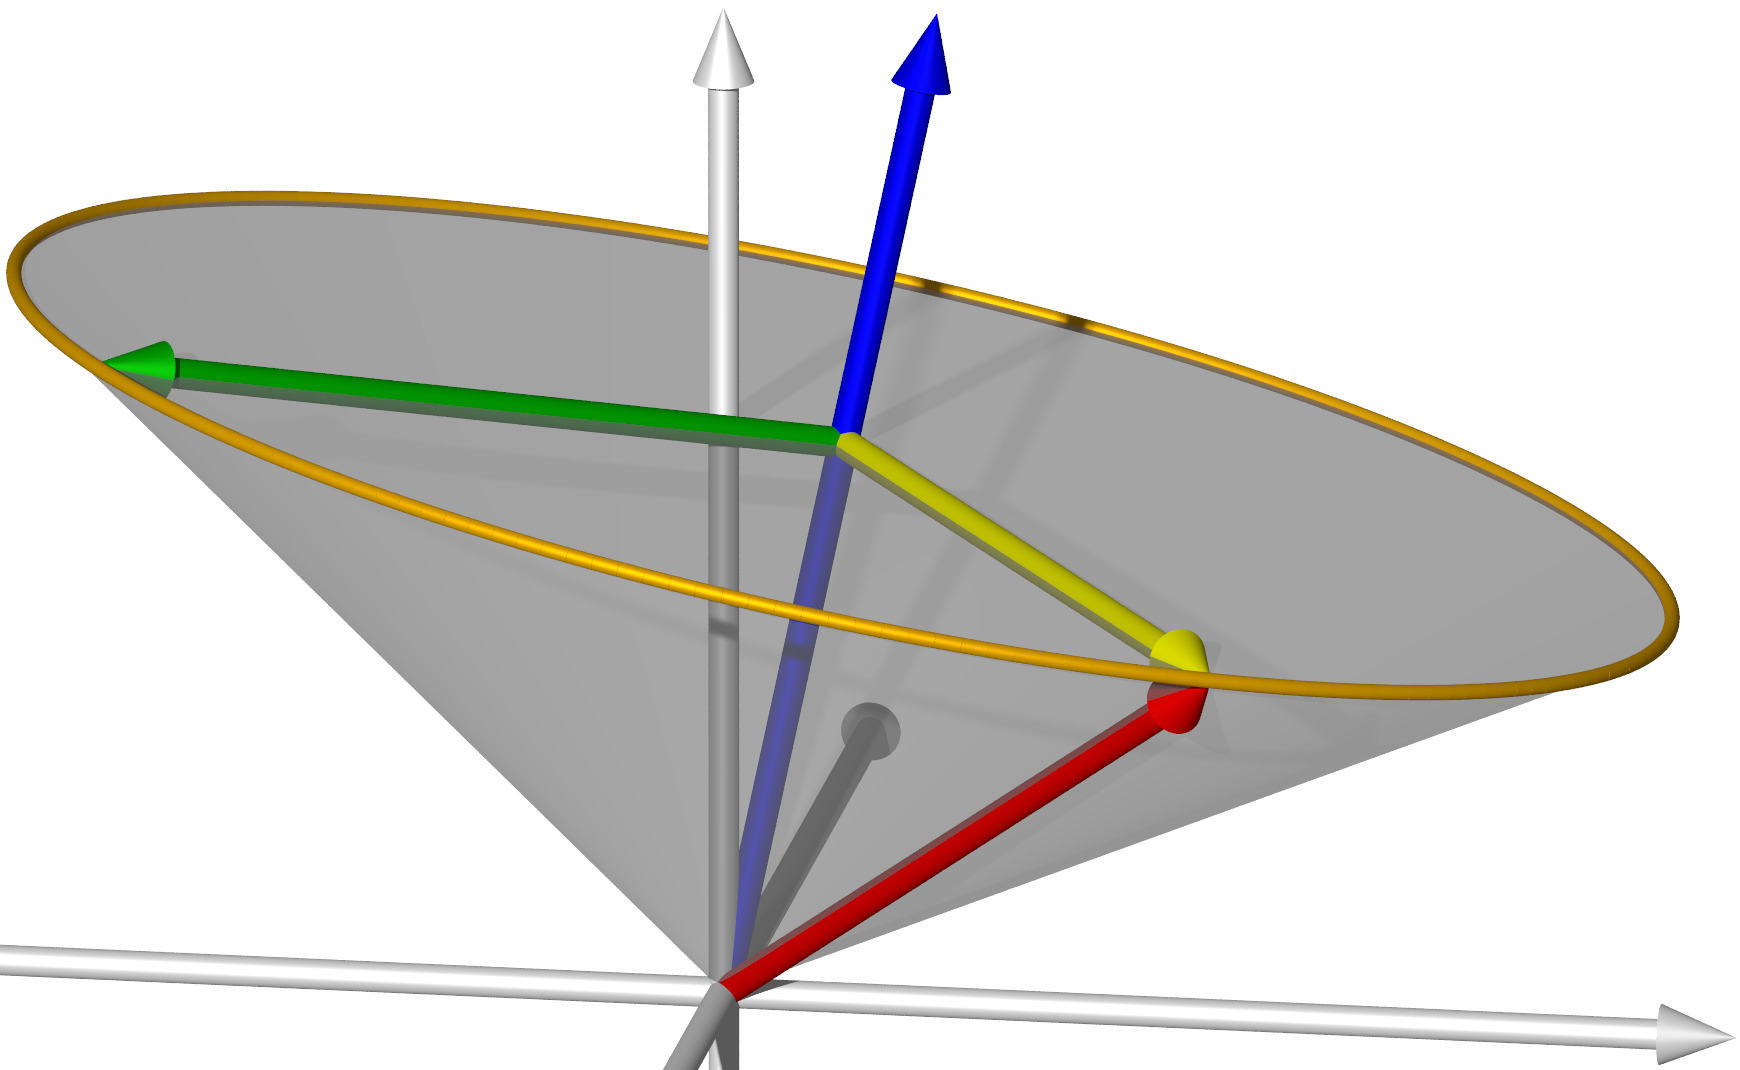
\includegraphics[width=\textwidth]{../slides/7/images/rodriguez.jpg}};
	\node[color=red] at (1.6,-0.9) {$\vec{x}$};
	\node[color=blue] at (0.5,2) {$\vec{k}$};
}
\uncover<11->{
	\node[color=darkgreen] at (-3,1.1) {$\vec{x}\times\vec{k}$};
}
\uncover<10->{
	\node[color=yellow] at (2.2,-0.2)
		{$\vec{x}-(\vec{x}\cdot\vec{k})\vec{k}$};
}
\end{tikzpicture}
\end{center}
\end{block}}
\end{column}
\end{columns}
\vspace{-15pt}
\uncover<5->{%
{\usebeamercolor[fg]{title}Dimension:} $\operatorname{SO}(3)$ ist eine
dreidimensionale Gruppe}
\end{frame}
\egroup
